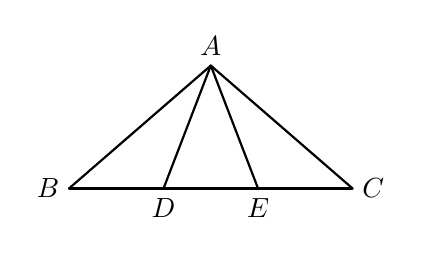
\begin{tikzpicture}[line cap=round,line join=round,scale=0.6]
% points on base BC with D,E trisecting: BD=DE=EC
\coordinate (B) at (0,0);
\coordinate (C) at (6,0);
\coordinate (D) at (2,0);
\coordinate (E) at (4,0);

% apex A (placed above between D and E, like the figure)
\coordinate (A) at (3,2.6);

% segments
\draw[thick] (B) -- (C);
\draw[thick] (A) -- (B);
\draw[thick] (A) -- (C);
\draw[thick] (A) -- (D);
\draw[thick] (A) -- (E);

% labels
\node[left]  at (B) {$B$};
\node[right] at (C) {$C$};
\node[below] at (D) {$D$};
\node[below] at (E) {$E$};
\node[above] at (A) {$A$};

\end{tikzpicture}